\chapter{Dataset}
\label{ch:dataset}

% Overall goals of chapter

% Explain what configuration/data is desired for the analysis.
% Explain that Science Park stations are going to be the focus.
% It is best suited because of high density of stations, and known configurations.
% Show what data is available to work with.
% Show that much of the data remains after cuts and will be used in the next chapter.
The dataset that will be used for the analysis in following chapters is presented here. The focus will be on a specific subset of stations. The initial raw dataset will be outlined. The quality requirements imposed on the data are then discussed. The resulting dataset that is used in the analysis is finally summed up.


\section{Dataset requirements for analysis}

% Direction reconstructions requires 3 or more stations (or detectors)
% Preferably triangular shape, at least not to much on a line.
% Stations must be close enough together (\SI{<1}{\kilo\meter}) to have lot of detections for statistics.
% Uptime must be good, specifically simultaneous uptime of stations.
% Properly configured station to make triggering similar.
At least three detection points are required for the reconstruction of the shower direction. More detections can be used to improve the accuracy. A temporal and structural analysis of the shower front will be performed and properties of the air shower will be reconstructed.

The detection points can either be individual \hisparc detectors or \hisparc stations. In order to suitable for accurate reconstructions the detection points must meet some criteria. They must be close enough to simultaneously detect air showers of the desired cosmic-ray energy. They should not all be on a single line, because that negatively affects the reconstruction accuracy.

The detection stations need to have been online simultaneously for extended periods of time. Simultaneous uptime increases the exposure time, which is needed to increase the chance of detecting the rarer very-high-energy cosmic rays. Moreover, many other coincidences between stations are required to calibrate the timing offsets.

Finally the stations must have been configured properly, moreover the locations of the detectors must be known. If the detector locations are unknown they could theoretically be as far as \SI{60}{\meter} from the \gps antenna location, though in practice this has never been the case. With the known location of the individual detectors each detector can be used separately in the reconstruction, or at least the center of mass location of the station detectors is known.


\section{Cluster selection}

% Possible clusters with close stations: Zaanlands/SciencePark/Twente/Eindhoven.
% Science Park for main analysis, because it has most potential for exploring the shower front. Highest sampling for each shower.
% All stations have 4 detectors and are capable of stand-alone reconstruction.
% Science park stations have good uptime.
% Mean/noise filter disabled for long period for good trigger time reconstruction.
% Large distance between outer detectors, detectors in between useful for accurate station timing offsets and more accurate reconstructions.
Over \num{100} combinations of \hisparc station pairs can be found in which the stations are separated by less than \SI{1}{\kilo\meter}. If combinations of three stations are desired in which each leg of the triangle is at most \SI{1}{\kilo\meter} a set of approximately \num{180} triangles are found, with some stations occuring in multiple triples.

From these triples there are \num{7} triples which are isolated, meaning that the \num{21} stations in those do not occur in other triples. However, in only \num{2} of these triples, University Twente and Zaanlands Lyceum, do the stations have a significant simultaneous uptime, known detector positions, and no known unknown configuration issues.

There are two station clusters, University Eindhoven and Amsterdam Zuid, in which four stations are close together and multiple combinations of triples can be made. However, some of the Amsterdam-Zuid stations have been moved when a school changed their location, and the previous detector positions have not been recorded properly. Additionally the simultaneous uptime is relatively low.

Finally there is the Amsterdam Science Park cluster. The Science Park cluster currently has \num{11} detection stations, a number which gradually grew over time. This cluster has a high simulteneous uptime and for each of these staitons the detector locations, including changes of time, are known. One of the Science Park stations, 507, is located within the main \nikhef building, the building above the detectors greatly attenuate the number of electrons and gammas. The acceptance and response of this station differs from other stations. This station will be ignored because the full effects of the attenuation are not yet understood, work on understanding this is on going [refrence LiO Gerrit].

So four possible candiate clusters remain, their layouts are shown in \ref{fig:compact_clusters}. For the analysis in this thesis the Amsterdam Science Park cluster will be used because it affords the most opportunities for detailed studies. The Science Park cluster is the only cluster with exclusively 4-detector stations. This allows for direction reconstruction within each station and such stations have a higher shower acceptance than 2-detector stations.

\begin{figure}
    \centering
    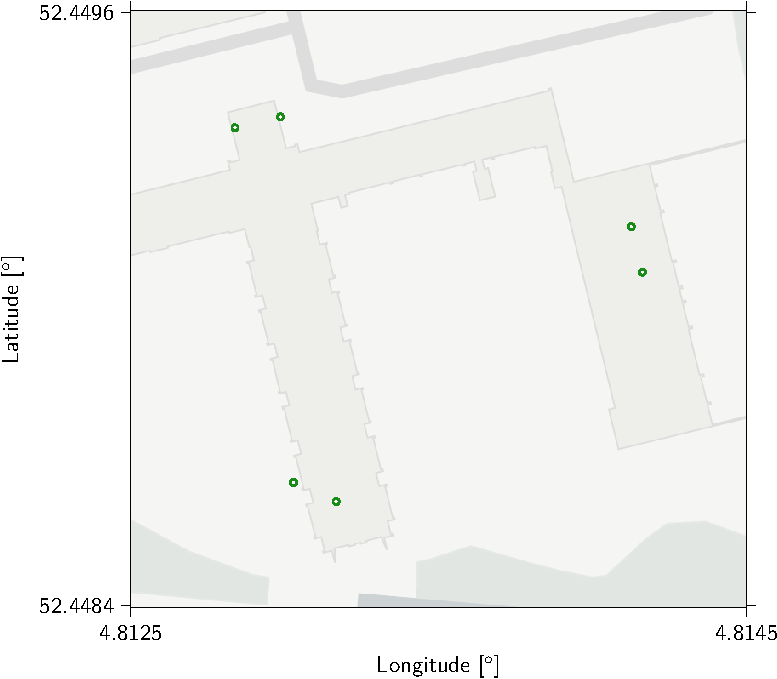
\includegraphics[width=0.23\linewidth]{plots/dataset/stations_102_104_105_detectors.pdf}
    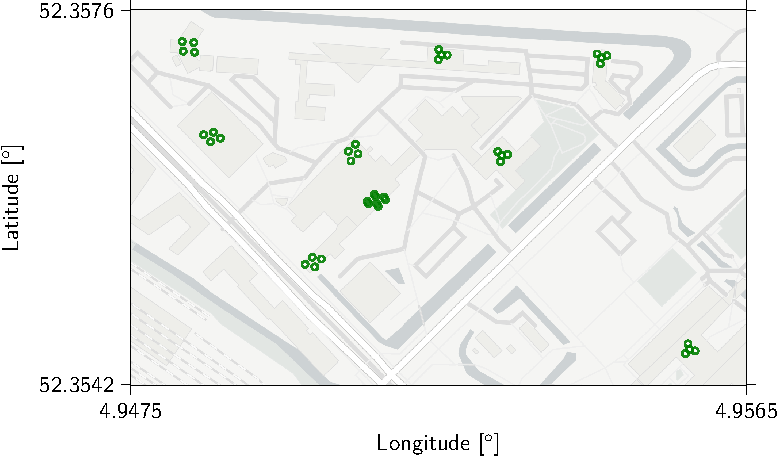
\includegraphics[width=0.23\linewidth]{plots/dataset/stations_501_502_503_504_505_506_508_509_510_511_detectors.pdf}
    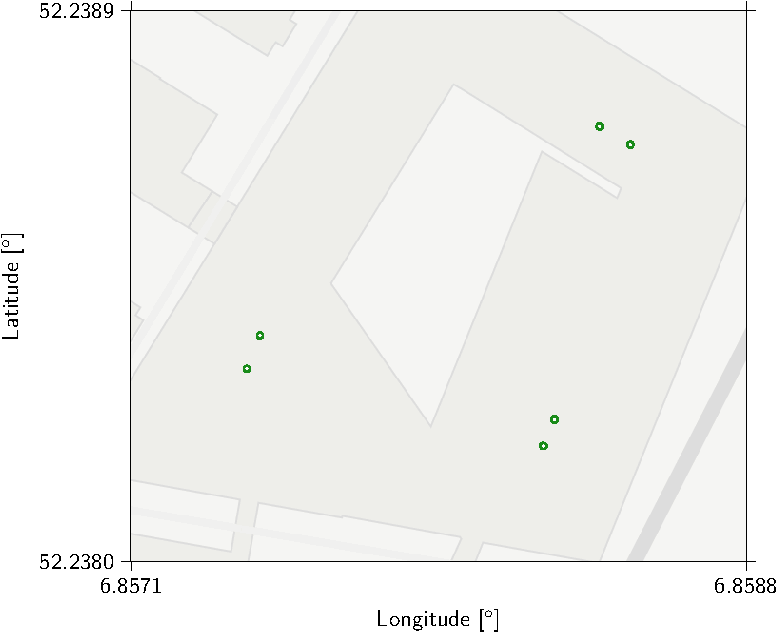
\includegraphics[width=0.23\linewidth]{plots/dataset/subcluster_7000.pdf}
    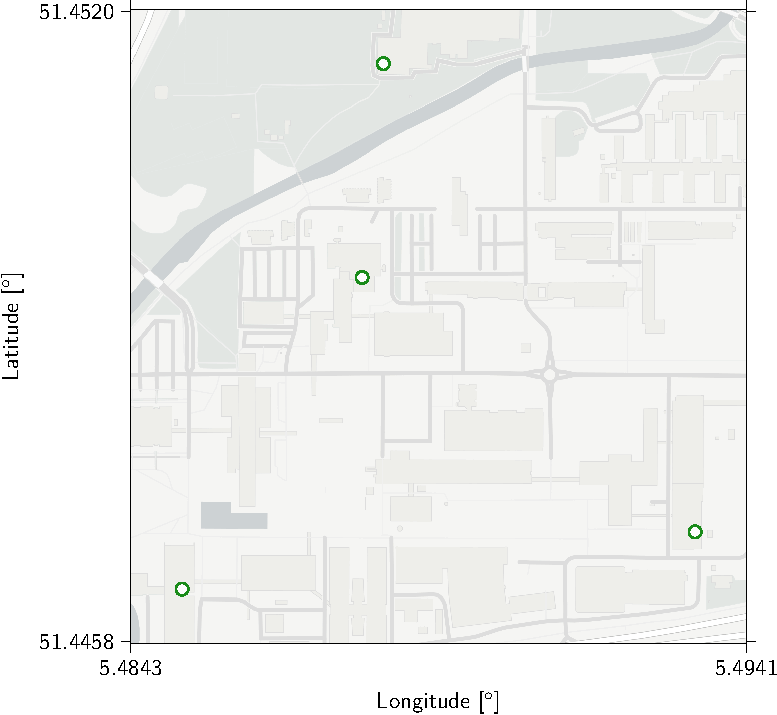
\includegraphics[width=0.23\linewidth]{plots/dataset/stations_8001_8004_8008_8009.pdf}
    \caption{Compact station clusters in the \hisparc network. From left to right are shown Zaanlands Lyceum, Science Park, University Twente, and University Eindhoven. Each presents excellent opportunities for reconstructions of showers. The overall layouts are fairly triangular and the stations are close enough to have many coincidences.}
    \label{fig:compact_clusters}
\end{figure}


\section{Raw data}

% Start date for each station and number of raw triggered events
Not all Science Park stations were deployed at the same time, several were installed during my research period. The first station at Science Park was station 501 which started data taking in March 2004. A year later a second station was installed at the University of Amsterdam. In August 2008 an additional five stations were added. Finally three more stations were added in 2013, 2014, and 2015. In \cref{tab:detected_events} the dates on which the stations started data taking is listed, also the total number of events recorded up to February 2016 [check] is shown. Station 507 is excluded for reasons stated above.

\begin{table}
    \centering
    \begin{tabular}{@{}llr@{}}
        \toprule
        Start date & Station & Number of events ($10^6$) \\
        \midrule
        2004-03-26 & 501     &                       220 \\
        2005-01-31 & 509     &                       120 \\
        2008-08-02 & 502     &                       120 \\
        2008-08-02 & 503     &                       130 \\
        2008-08-02 & 504     &                       150 \\
        2008-08-03 & 506     &                        80 \\
        2008-08-07 & 505     &                       120 \\
        2013-06-17 & 508     &                        30 \\
        2014-09-29 & 510     &                        30 \\
        2015-06-16 & 511     &                        10 \\
        \bottomrule
    \end{tabular}
    \caption{The number of detected events in the Science Park stations between their start date and 2017-02-01.}
    \label{tab:detected_events}
\end{table}

The total number of events does not scale linearly with time since first data taking. This is caused by station and detector downtime, and slightly differing trigger rates due to calibration and construction differences. The raw data also includes triggered events due to background radiation. Background radiation includes EAS with only very few or single particles at ground level.


\section{Data quality cuts}

% Cut based on date to use data after 2011-6 to ensure GPS time is used, instead of UTC time.
% Cut days on which configuration changed.
% Cut station or detector for entire day or single event, show examples of cuts for various parameters.
% If detector is working badly, better to exclude for entire day, and ignore it for particle density.
% Check that bad data does not introduce unwanted bias.
Not all of the events which were counted in \cref{tab:detected_events} will be taken into account for the analysis. Data quality cuts will be performed prior to the further analysis. Some quality criteria were discussed in \cref{sec:data_quality_criteria}.


\subsection{Mixed \utc and \gps timestamps}

Originally the \gps module in the \hisparc electronics was configured to use \utc timestamps during data taking, around March 2010 the default configuration was changed to use \gps timestamps. The value of this configuration setting is unfortunately not included in the stored configuration messages from stations, so the chosen setting can not be recovered easily. Research into coincidences with lightning strikes has shown that not all \hisparc stations were simultaneously reconfigured to \gps time. The research showed that by June 2011 no significant number of stations were still on \utc time. If the time settings between a pair of stations do not match the number of coindcidences will be less than expected. By offsetting event timestamps by the number of active leap seconds and comparing the coincidence rate again it might be possible to determine which station is using the wrong setting. Only events after June 2011 will be considered.


\subsection{Configuration changes}

Days on which the configuration of a station is changed will also be ignored. On such days the station will be operating under different configurations for various parts of the day. For example, if at noon the \pmt voltages were changed the \mpv value for the affected detectors may have changed. The \mpv is determined daily using all data of that day, but that data will contain mixed datasets in the fit, resulting in a bad calibration. The total number of days skipped because of this is relatively small. Some of the days with a new configuration have only partial data because the station may have been restarted and reconfigured after a longer downtime. In table \cref{tab:changed_parameters} the number of days on which a setting was changed for a station is shown. Also the total number of days of data to be excluded per station is shown. Station 501 has most days with changes because it was often used to test new software, or at times its \gps was borrowed by another station.

\begin{table}
    \centering
    \begin{tabular}{@{}lrrrrrrrrrr@{}}
        \toprule
        Parameter     & 501 & 502 & 503 & 504 & 505 & 506 & 508 & 509 & 510 & 511 \\
        \midrule
        \gps position &  23 &   8 &   7 &   4 &  11 &   3 &   1 &   4 &  10 &   1 \\
        Electronics   &   3 &   3 &   1 &   1 &   2 &   3 &   2 &   1 &   0 &   0 \\
        \pmt voltages &  21 &  16 &  23 &  17 &  23 &  12 &   6 &   6 &   8 &   2 \\
        \midrule
        Total days    &   ? &   ? &   ? &   ? &   ? &   ? &   ? &   ? &   ? &   ? \\
        %[number of unique days to be excluded]
        \bottomrule
    \end{tabular}
    \caption{The number of days on which configuration or hardware changes were made to the Science Park stations. The last row lists the total days excluded, since on some days multiple changes were made to the same stations.}
    \label{tab:changed_parameters}
\end{table}


\subsection{Drastic unexpected calibration value changes}

Most calibration values are determined daily, for the station offset data from days before and after the concerning date is also used. Normally the calibration values differ little from day to day. Many large changes coincide with changes to the station or detector configurations. The remaining calibration changes are in most cases caused by external effects such as the replacement of signals cables or \pmts. Such changes are generally not logged, making it hard to reconstruct what happened. Days on which a calibration value changes significantly will also be excluded to prevent bad data due to unaccounted for changes to a station. In \cref{fig:mpv} the daily determined \mpv for each detector in each station is shown. The visible jumps often coincide with changes to the \pmt voltage calibration, and are therefore already excluded. The days of the remaining jumps will also be excluded. In most cases the \mpv does seem to settle to a stable value after a jump. Except for station 501 the \gps location of the Science Park stations only changed by up to \SI{2}{\meter}. However, for station 501 the \gps location has jumps of up to \SI{25}{\meter}, this is explained by the temporary \gps antenna it used for a period of time, while its normal \gps antenna was used for a test. In this case we know the causes of the jumps.
% and also that the temporary \gps had a bad sky coverage, and therefore less accurate timing. It's events recorded during that period will be excluded.

[Analysis: find significant outliers (determine criteria), determine which (and how many) days are affected (after previous cuts)]

\begin{verbatim}
    changed param   501 502 503 504 505 506 508 509 510 511
    mpv             ?   ?   ?   ?   ?   ?   ?   ?   ?   ?
    offset          ?   ?   ?   ?   ?   ?   ?   ?   ?   ?
    GPS             ?   ?   ?   ?   ?   ?   ?   ?   ?   ?
    Total days      [number of unique days to be excluded]
\end{verbatim}

\begin{figure}
    \centering
    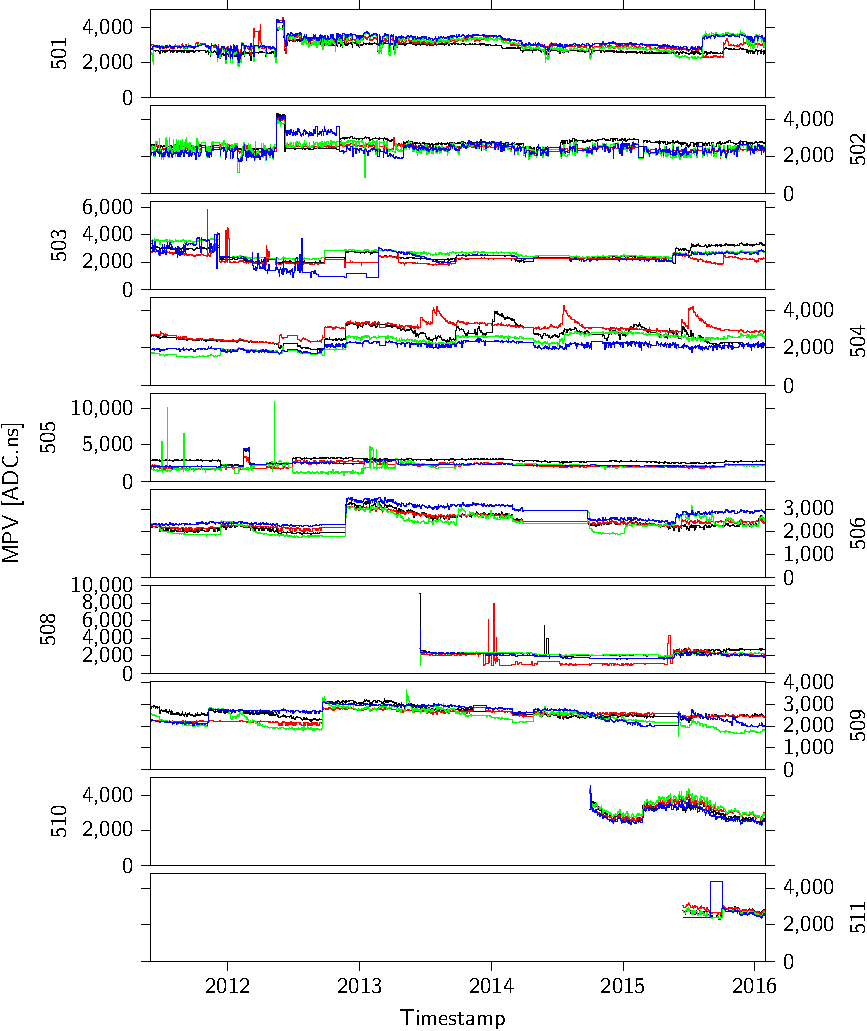
\includegraphics[width=0.7\linewidth]{plots/dataset/mpv.pdf}
    \caption{Timelines of the calibrated \mpv of each detector for the Science Park stations. These values are determined daily. Large jumps are likely to due to recalibration or replacement of \pmts.}
    \label{fig:mpv}
\end{figure}


\subsection{Failed reconstruction of observables in events}

If a detector part of an event has a bad baseline the detector will be excluded for that event, if the trigger reconstruction failed the entire event is excluded, if the \mpv fit or timing offset of a detector fails for a day that detector is excluded for the entire day, and if the station timing offset fails the station is excluded for the entire day.

Additionally if the number of events on a day in which a specific detector would be excluded exceeds a nominal fraction it will be considered malfunctioning and excluded for the entire day. Similarly for a station, if too many events of a station are excluded on a day the station will be excluded for the entire day. If the mean filter \cref{ssec:mean_filter} is enabled on a station then a failed trigger time reconstruction is expected for approximately \SI{0.1}{\percent}. With the mean filter disabled over a magnitude less failed reconstructions are expected. Failed reconstructions can still occur due to back to back triggers, which can interfere with the trigger reconstruction algorithm.

\begin{figure}
    \centering
    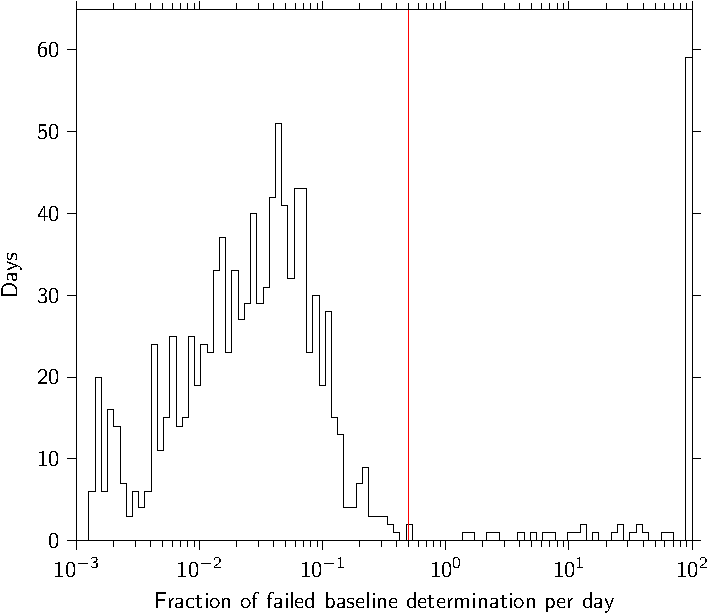
\includegraphics[width=0.7\linewidth]{plots/dataset/histogram_failed_baseline_504_4.pdf}
    \caption{Histogram of fraction of failed baseline determinations per day for a detector for station 504. Up to \SI{0.5}{\percent} appears normal, higher indicates problem with the detector and it may be best to exclude it for the entire day.}
    \label{fig:bad_baseline}
\end{figure}

\begin{figure}
    \centering
    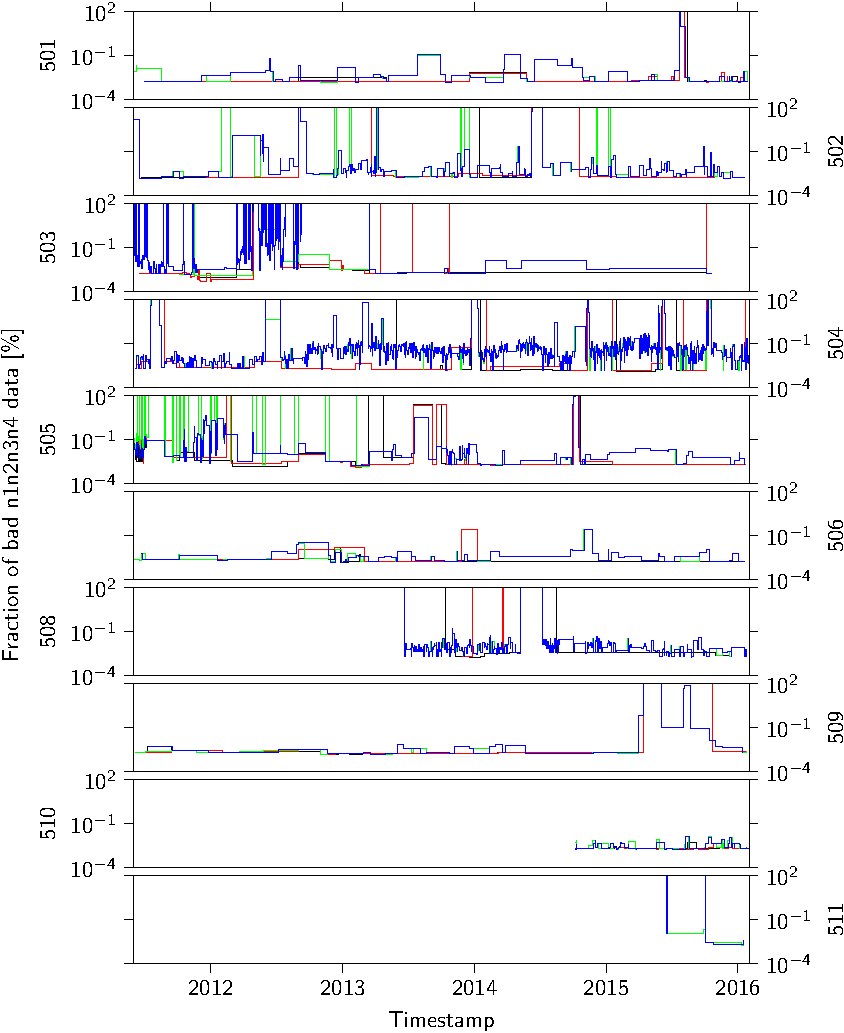
\includegraphics[width=0.7\linewidth]{plots/dataset/bad_fraction_n1n2n3n4.pdf}
    \caption{If bad fraction is higher than \SI{.5}{\percent} discard the detector for entire day. If below, exclude only that detector for those events.}
    \label{fig:bad_n}
\end{figure}

[Add table of observables+thresholds or add threshold lines to plots]


\section{Remaining uptime and events per station}

% Graph uptime of remaining events
% time with n simultaneaous active stations
The cuts discussed above are applied to the data of the individual stations. In \cref{tab:remaining_events} the remaining number of days with data and number of events are shown. These events have not been filtered based on being able to successfully reconstruct the shower.

\begin{table}
    \centering
    \begin{tabular}{@{}llr@{}}
        \toprule
        Station & Days with data & Number of events ($10^6$) \\
        \midrule
        501     & ?              &                        97 \\
        502     & ?              &                        66 \\
        503     & ?              &                        71 \\
        504     & ?              &                        86 \\
        505     & ?              &                        70 \\
        506     & ?              &                        76 \\
        508     & ?              &                        32 \\
        509     & ?              &                        82 \\
        510     & ?              &                        24 \\
        511     & ?              &                         8 \\
        \bottomrule
    \end{tabular}
    \caption{The number of remaining days with events and the total number of remaining events for the Science Park stations.}
    \label{tab:remaining_events}
\end{table}


\section{Effect on coincidences}

Removing bad events also affects the number of coincidences. Interesting for the purpose of calibrations, mainly station timing offsets, is the number of coincidences in which at least 2 stations are in coincidence. In the remaining dataset there are \num{13391318} coincidences with at least 2 stations in coincidence. The largest potion of this is dominated by the stations which are close together, i.e 501 and 510. When more stations in coincidence are required, for more accurate reconstruction, the number of coincidences sharply drops. This is because the distances to the other stations are much larger and much larger air showers are required to create the coincidences, and because more stations are required to have been active simultaneously. In \cref{tab:remaining_coincidences} the number of coincidences before and after the cuts with at least N stations are listed.

\begin{table}
    \centering
    \begin{tabular}{@{}lrr@{}}
        \toprule
        N  & Before cut & After cut \\
        \midrule
         3 &    1975275 &         ? \\
         4 &     544342 &         ? \\
         5 &     187480 &         ? \\
         6 &      71286 &         ? \\
         7 &      27552 &         ? \\
         8 &       9714 &         ? \\
         9 &       3111 &         ? \\
        10 &        787 &         ? \\
        \bottomrule
    \end{tabular}
    \caption{The number of coincidences before and after the quality cuts between the Science Park stations.}
    \label{tab:remaining_coincidences}
\end{table}


\section{Remaining data}

The remaining data contains only data for which the offline calibration was successful, and only data from days on which the station was not reconfigured. As mentioned the largest fraction of 2-station coincidences are those of station 501 and 510.

The single station events in the dataset may still be unreconstructable, or appear to be accidental triggers. However, in some cases they are part of the outer regions of large showers, where the shower core is closer to other stations. In such cases the events should be accounted for when reconstructing the shower using data from the multiple stations. That means that for events in coincidences the events themselves may not be reconstructable, but when taken together they can be.
